 \documentclass{beamer}

\usetheme{MagdeburgFIN}
\usefonttheme{structurebold}
\usepackage{graphicx}
\usepackage{float}
\usepackage{url}
\usepackage{pdfpages}


\title{Advanced Topics in Machine Learning Programming Task}
\author{Jannis Becke, Christian Lausberger and Maik Riestock}
\date{June 22, 2015}
\institute{Advanced Topics in Machine Learning}

\begin{document}

\begin{frame}[plain]
 \titlepage
\end{frame}

\begin{frame}
\frametitle{Data Preparation}

49 Attributes, ~101.000 Instances

Reasons for attribute removal:
\begin{enumerate}
\item \textbf{Uniqueness}

\item \textbf{Missing Values}

\item \textbf{Unequal Distribution}

\item \textbf{Single Attribute}
\end{enumerate}
No instance was removed
\end{frame}


\begin{frame}
\frametitle{Choice of Algorithms}
Algorithms:
\begin{itemize}
 \item Naive Bayes
 \item SVM
 \item YATSI
 \item Decision Table
\end{itemize}
\end{frame}

\begin{frame}
\frametitle{Implementation}
Choice of libraries:
\begin{itemize}
 \item weka
 \item libSVM
 \item collectiveClassifiers
\end{itemize}
\end{frame}

\begin{frame}
\frametitle{Settings}
Decision Table:
\begin{itemize}
 \item Search: Best First 
 \item Evaluation Measure: accuracy/RMSE
\end{itemize}

SVM:
\begin{itemize}
 \item Type: C-SVM
 \item Kernel: radial basis function
 \item with normalizing, no weights
\end{itemize}

YATSI:
\begin{itemize}
 \item KNN: 15
\end{itemize}
\end{frame}

\begin{frame}
\frametitle{Experiments}
Settings:
\begin{itemize}
 \item Percentage Split / Cross-Validation
 \item Accuracy of classification as quality measure
 \item two additional data sets:
 \begin{itemize}
 	\item even class dataset (equally distributed classification attribute)
 	\item two class dataset (join label $>30$, $<30$)
 \end{itemize}
\end{itemize}
\end{frame}

\begin{frame}
\frametitle{Results}
	\begin{figure}
		\center
		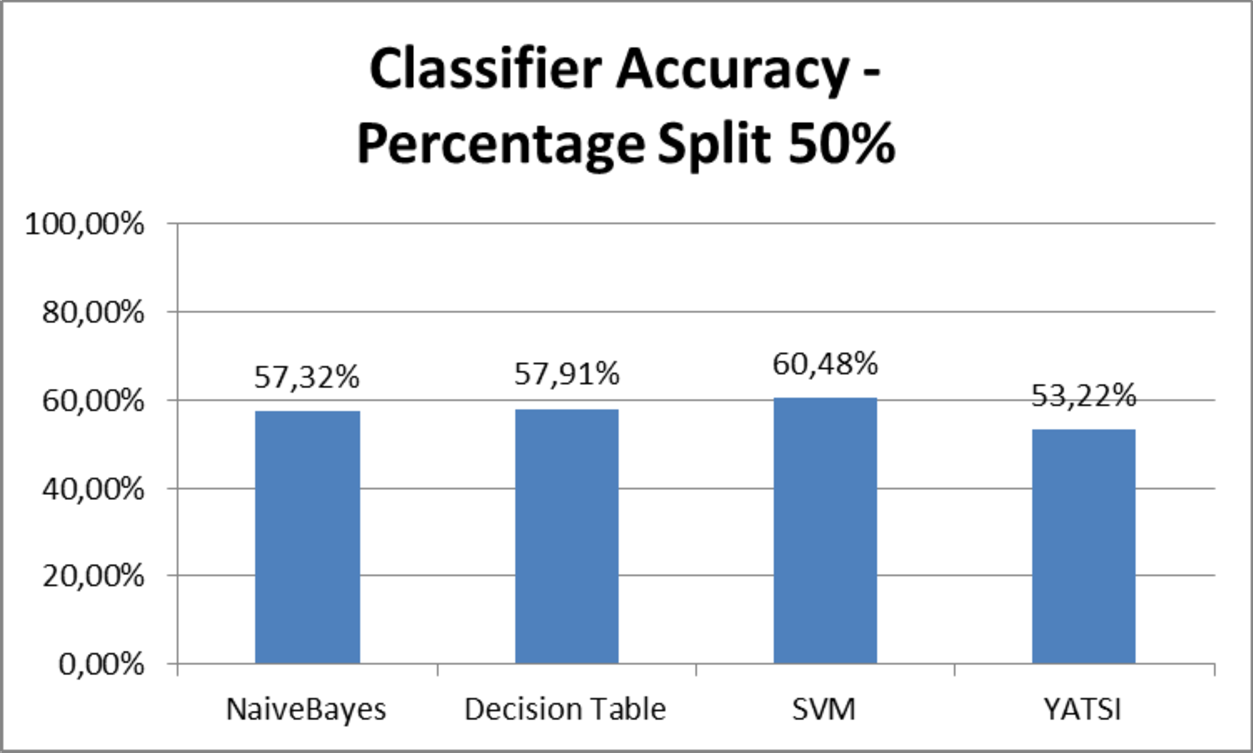
\includegraphics[width=.8\textwidth]{./img/Accuracy_PS50.pdf}
	\end{figure}
\end{frame}
\begin{frame}
	\frametitle{Results}
	\begin{figure}
		\center
		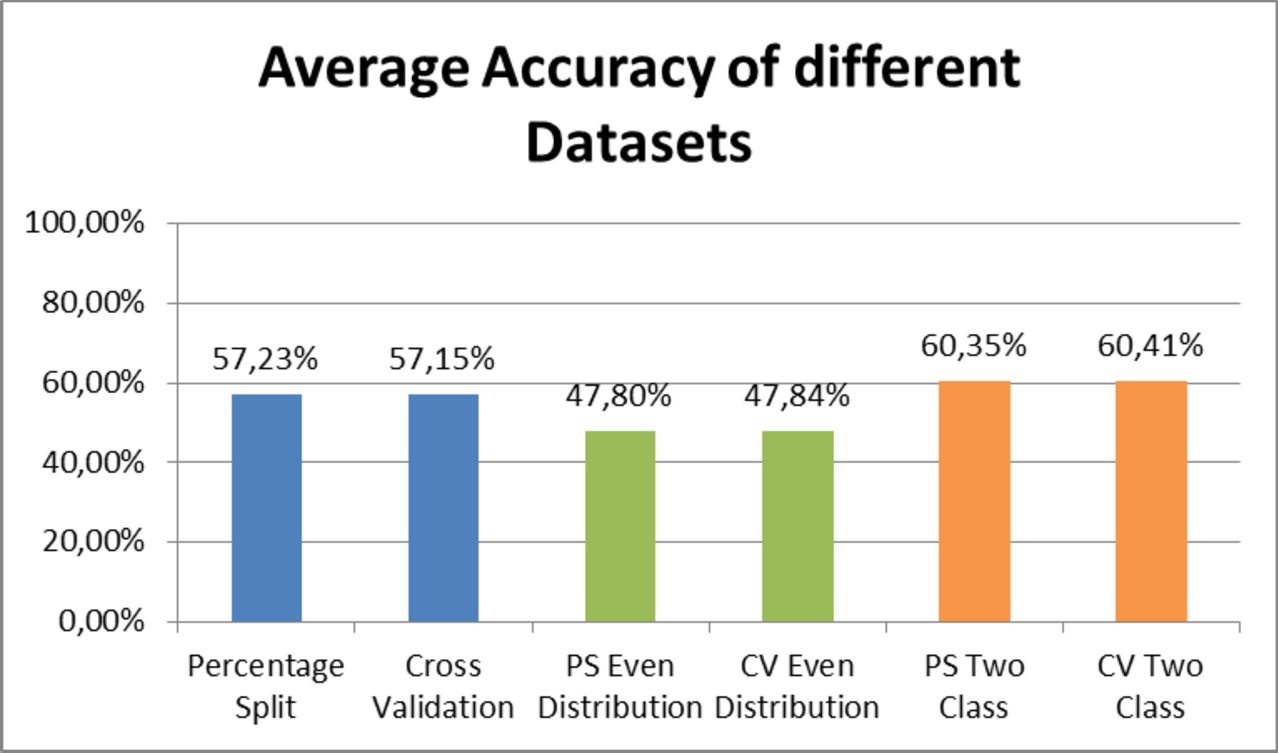
\includegraphics[width=.8\textwidth]{./img/avgAccuracy.pdf}
	\end{figure}
\end{frame}
\begin{frame}
	\frametitle{}
	\centering
	{\Large \textbf{Thanks for Your attention!}}
\end{frame}
\begin{frame}
	\begin{figure}
		\center
		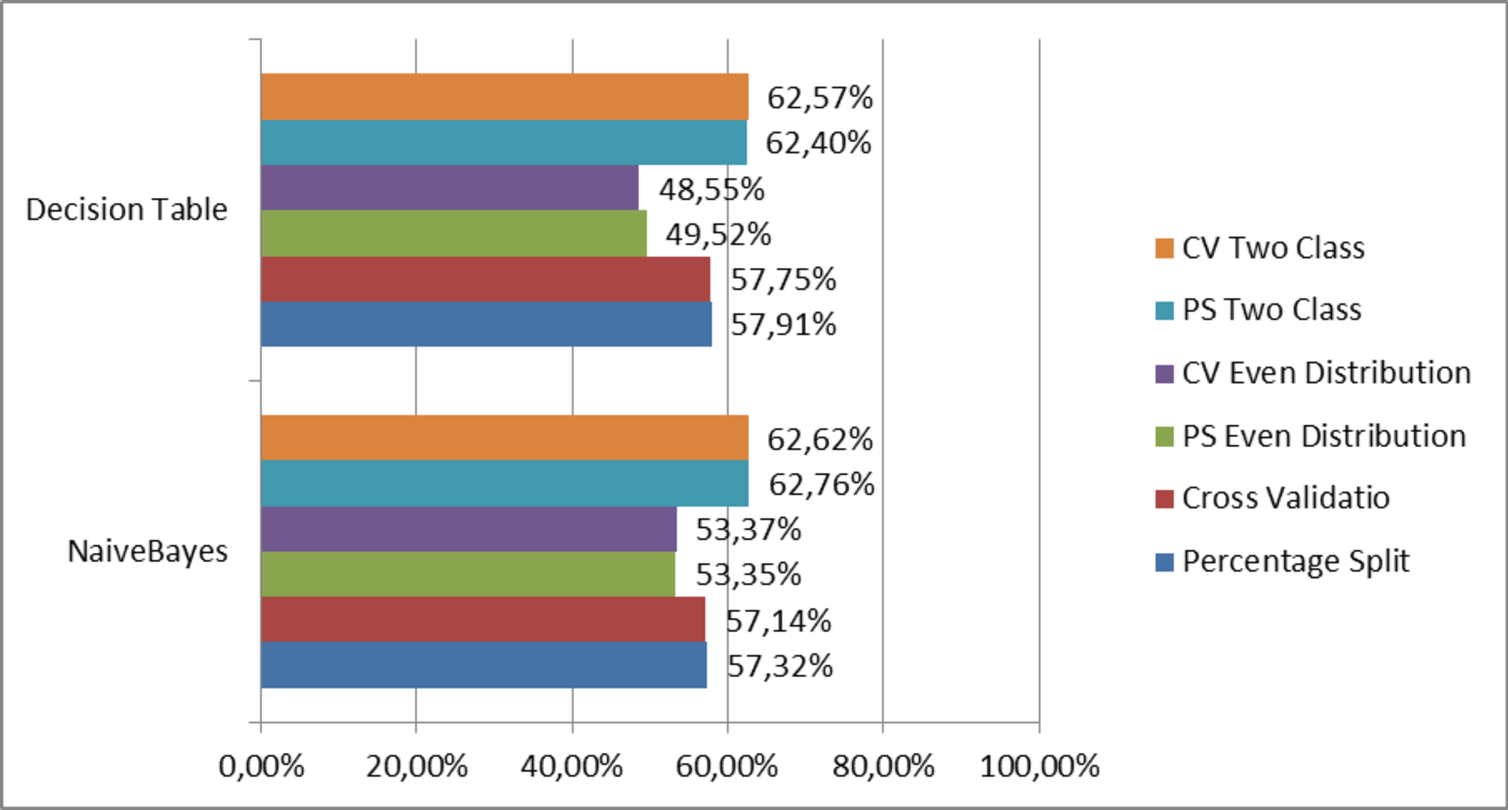
\includegraphics[width=.8\textwidth]{./img/Accuracy1.pdf}
		\end{figure}
\end{frame}
\begin{frame}
	\begin{figure}
		\center
		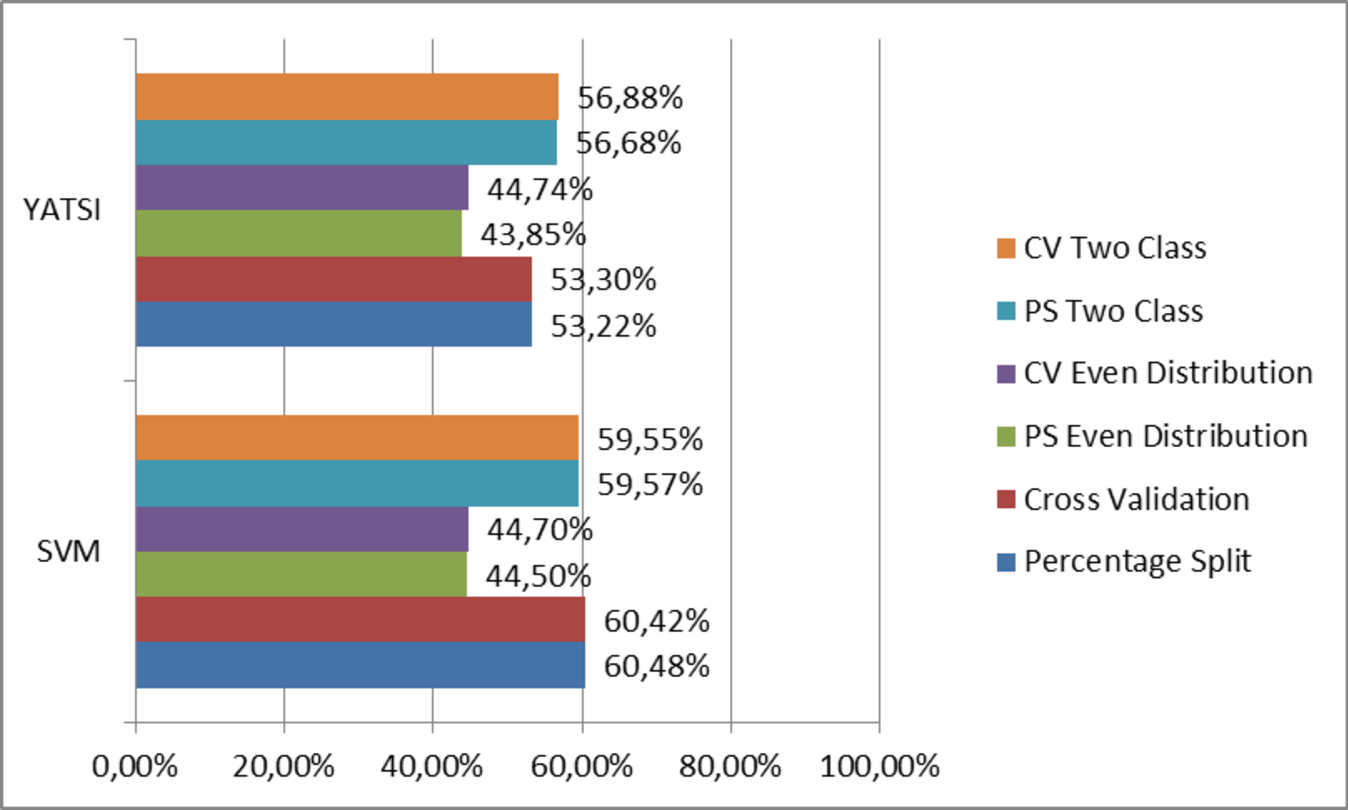
\includegraphics[width=.8\textwidth]{./img/Accuracy2.pdf}
		\end{figure}
\end{frame}
\end{document}
